% MATH 578 HW1
% LUKE WUKMER

\documentclass[12pt]{article}

% note: some of these are extremely useful and i don't remember why :o
%\usepackage{savetrees} % disable custom geometry stuff if you do this
\usepackage{titling}    % contol over title & stuff
\usepackage{amsmath, amsthm, amssymb, amsfonts}
\usepackage{amsxtra, amscd, geometry, graphicx}
\usepackage{endnotes}
\usepackage{cancel}
\usepackage{wrapfig}    %inline figs
\usepackage{bm} %allows fancy stuff like bold greek in math mode
\usepackage{alltt}
\usepackage{enumerate} %more/easier control over lists, also see enumitem
%\usepackage[all,cmtip]{xypic}
\usepackage{mathrsfs}
\usepackage{listings} % code with syntax highlighting etc
\usepackage{caption}
\usepackage[raggedright]{sidecap} % side captions
\usepackage{tabu}     % more customizable tables
%\usepackage{subfigure}
%\usepackage{subcaption}
%\usepackage[pdftex]{hyperref}
%\usepackage[dvips,bookmarks,bookmarksopen,backref,colorlinks,linkcolor={blue},citecolor={blue},urlcolor={blue}](hyperref}

\graphicspath{ {./figs/} }

\usepackage{color}


\definecolor{mygreen}{rgb}{0,0.6,0}
\definecolor{mygray}{rgb}{0.5,0.5,0.5}
\definecolor{mymauve}{rgb}{0.58,0,0.82}

\lstset{ %
basicstyle=\footnotesize,        % the size of the fonts that are used for the code
%breakatwhitespace=false,         % sets if automatic breaks should only happen at whitespace
breaklines=false,                 % sets automatic line breaking
captionpos=t,                    % sets the caption-position to bottom
commentstyle=\color{mygray},    % comment styleh
%  deletekeywords={...},            % if you want to delete keywords from the given language
%  escapeinside={\%*}{*)},          % if you want to add LaTeX within your code
%  extendedchars=true,              % lets you use non-ASCII characters; for 8-bits encodings only, does not work with UTF-8
frame=single,                      % adds a frame around the code
%keepspaces=false,                 % keeps spaces in text, useful for keeping indentation of code (possibly needs columns=flexible)
% columns=flexible,
  keywordstyle=\color{blue},       % keyword style
  language=Python,                 % the language of the code
%  otherkeywords={*,...},           % if you want to add more keywords to the set
%  numbers=left,                    % where to put the line-numbers; possible values are (none, left, right)
%  numbersep=5pt,                   % how far the line-numbers are from the code
%numberstyle=\tiny\color{mygray}, % the style that is used for the line-numbers
%  rulecolor=\color{black},         % if not set, the frame-color may be changed on line-breaks within not-black text (e.g. comments (green here))
showspaces=false,                % show spaces everywhere adding particular underscores; it overrides 'showstringspaces'
showstringspaces=false,          % underline spaces within strings only
%  showtabs=false,                  % show tabs within strings adding particular underscores
%  stepnumber=2,                    % the step between two line-numbers. If it's 1, each line will be numbered
  stringstyle=\color{mymauve},     % string literal style
%  tabsize=2,                      % sets default tabsize to 2 spaces
title=\lstname                   % show the filename of files included with \lstinputlisting; also try caption instead of title
}
% change up the fonts (pick one only)
%\usepackage{times}%
%\usepackage{helvet}%
\usepackage{palatino}%
%\usepackage{bookman}%


% These are italic.
% \theoremstyle{definition}

% These are normal (i.e. not italic).
\theoremstyle{definition}

%\newtheorem{prob}{Problem}[section]
\newtheorem{prob}{Problem}
\newtheorem*{prob*}{Problem}
\newtheorem*{soln*}{Solution}
\newtheorem{soln}{Solution}


% New Commands: Common Math Symbols
\providecommand{\R}{\mathbb{R}}%
\providecommand{\N}{\mathbb{N}}%
\providecommand{\Z}{{\mathbb{Z}}}%
\providecommand{\sph}{\mathbb{S}}%
\providecommand{\Q}{\mathbb{Q}}%
\providecommand{\C}{{\mathbb{C}}}%
\providecommand{\F}{\mathbb{F}}%
\providecommand{\quat}{\mathbb{H}}%

% haha, i originally forked this template from one provided by my abstract
% algebra TA (back in 2012 or something). probably don't need most of these,
% huh. 

% New Commands: Operators
%\providecommand{\Gal}{\operatorname{Gal}}%
%\providecommand{\GL}{\operatorname{GL}}%
%\providecommand{\card}{\operatorname{card}}%
%\providecommand{\coker}{\operatorname{coker}}%
%\providecommand{\id}{\operatorname{id}}%
%\providecommand{\im}{\operatorname{im}}%
%\providecommand{\diam}{{\rm diam}}%
%\providecommand{\aut}{\operatorname{Aut}}%
%\providecommand{\inn}{\operatorname{Inn}}%
%\providecommand{\out}{{\rm Out}}%
%\providecommand{\End}{{\rm End}}%
%\providecommand{\rad}{{\rm Rad}}%
\providecommand{\rk}{{\rm rank}}%
%\providecommand{\ord}{{\rm ord}}%
%\providecommand{\comp}{{\text{ $\scriptstyle \circ$ }}}%
\providecommand{\cl}[1]{\overline{#1}}%
\providecommand{\tr}{{\sf trace}}%
\providecommand{\spn}{{\rm span}}%

\renewcommand{\tilde}[1]{\widetilde{#1}}%
%\numberwithin{equation}{section}

% i like the squiggly ones more. add as needed

\renewcommand{\Psi}{\varPsi}

\newcommand*\rfrac[2]{{}^{#1}\!/_{#2}}

% a very fancy dot product \ip{f}{g}
\newcommand\ip[2]{ \left\langle {#1} , {#2} \right\rangle }

% "s.t." for math mode
\providecommand{\st}{\text{ s.t. }}

% \norm{f} and such, super useful
\newcommand{\norm}[1]{\left\lVert#1\right\rVert}

% determinant
%\newcommand{\det}[1]{\textsf{det}\left(#1\right)}

% jacobian
\providecommand{\J}{\textsf{J}}

% this makes the spacing between lines of font a little bigger
%\newcommand{\spacing}[1]{\renewcommand{\baselinestretch}{#1}\large\normalsize}
%\spacing{1.2}

\DeclareMathOperator*{\argmin}{arg\,min}
\DeclareMathOperator*{\argmax}{arg\,max}

\newcommand*\mcol[1]{\overset{\big\uparrow}{\underset{\big\downarrow}{#1}}}

% Makes the margin size a little smaller, i gots stuff to say
\geometry{letterpaper,margin=.8in}

% titling stuff (from package titling)
\posttitle{\par\end{center}}
\setlength{\droptitle}{-.5in}
% END PREAMBLE %%%%%%%%%%%%%%%%%%%%%%%%%
%%%%%%%%%%%%%%%%%%%%%%%%%%%%%%%%%%%%%%%%


\begin{document}

\title{Math 578 HW\textsuperscript{\#}2}
\author{Luke Wukmer}
\date{Fall 2016}
\maketitle \thispagestyle{empty} % remove the page number from the first page


%%%% PROBLEM 1

\begin{prob} QR via Givens rotations

    \begin{enumerate}[\bfseries(a)]
        \item
            An algorithm for QR decomposition of a tridiagonal matrix via Givens rotations is given in
            \texttt{givens.py} and \textbf{Appendix A}.
        \item
            Flop count for forming $R$ within Givens QR, using tridiagonal input $A$:
            \begin{enumerate}
                \item 6 flops per computing components $c,s$ of Givens rotation
                \item 1 application of $2\times2$ Givens matrix by $2\times3$ subblock.
                    Can calculate as 3 matrix-vector multiplications or $3(2mn-2)$ where $m,n=2$.
                    Or direct counting $\rightarrow 6\cdot3 = 18$ flops.
                \item (a)-(b) are repeated for each diagonal element except for the last two,
                    so $(n-2)$ times. On the second-to-last diagonal element,
                    the subblock to apply the Givens matrix to is only $2\times2$, instead of $2\times3$.
                    Using the logic above, this particular iteration requires $2\cdot6$ iterations
                    (plus the 6 in part (a)).
                \item
                    For the very last diagonal element, nothing changes.
            \end{enumerate}

                    Therefore, total flop count is
                    \begin{align*}
                        (6\cdot3 + 6)\cdot(n-2) + (6\cdot2 + 6) &= 24(n-2) + 18 \\
                                                                &= \mathcal{O}\left(n\right)
                    \end{align*}
        \item The matrix begins as tridiagonal. Givens rotations only will interact with nonzero columns
            of the $2\times n$ subblock relevant to each diagonal, which is only the first three.
            Thus, the only element above the first superdiagonal which may be influence by our QR algorithm
            is the single entry of the 2nd superdiagonal, which appears as the upper-right element of each
            2x3 subblock. Of course, our QR decomposition will make $R$ upper triangular, so all subdiagonals
            will be zeroed. Therefore, $R$ will in general have only nonzero elements on its main diagonal,
            as well as its first and second superdiagonals.
    \end{enumerate}
\end{prob}

\clearpage
%\dotfill % . . . . . . . . . . 
\hrulefill % ___________________________________________________________
%%%% PROBLEM 2
\begin{prob} Solving Least Squares Problems with QR.
    Relavant code to this problem is located in
    \texttt{lsq\_demo.py} and in the \textbf{Appendix}.
    \begin{enumerate}[\bfseries(a)]

        \item Backsubsitution to solve a upper triangular system $Rx=b$ is implemented in
            the function \texttt{lsq\_demo.back\_substitution(\dots)}.

        \item The above method was used to solve the linear systems described in Problem 2. These systems
            were generated using \texttt{A,b = lsq\_demo.demo\_system(n)} for $n = 5,6,\ldots,25$.
            Using back-substitution only (since $A$ as described is upper-triangular), we
            calculate the relative residual error of our solution $x$ via
            \[
                    e_n := \frac{\norm{Ax - b}_2}{\norm{b}_2}
                \]

        \item We solve the same system by finding the solution $x$ to $A^TA x = A^Tb$. This is found using
            Givens QR, as the system $A^TA$ is tridiagonal.
            We then calculate the relative residual error of \textit{this} solution $\tilde{x}$ as:
            \[
                    f_n := \frac{\norm{A\tilde{x} - b}_2}{\norm{b}_2}
                \]

        \item
Upon running, \texttt{lsq\_demo.py} generated the following output:
\begin{small}
\begin{verbatim}
n       e_n (backsub)           f_n (normal eqs)
-------------------------------------------------
5       3.43990022796e-16       2.40844199509e-14
6       3.62597321469e-16       9.21161907519e-14
7       3.75323885184e-16       3.44218058155e-13
8       3.84592537277e-16       1.29128889592e-12
9       3.9164986973e-16        4.89224891546e-12
10      3.9720546452e-16        1.85749088174e-11
11      4.01693804323e-16       7.08914229515e-11
12      4.05396129633e-16       2.71605924855e-10
13      4.08502658814e-16       1.04400239547e-09
14      4.11146716571e-16       4.02453325848e-09
15      4.13424555146e-16       1.55530155125e-08
16      4.15407418106e-16       6.02382571746e-08
17      4.17149175925e-16       2.33763354402e-07
18      4.18691322316e-16       9.08711126433e-07
19      4.2006633857e-16        3.53787365819e-06
20      4.21300016229e-16       1.37928389734e-05
21      4.22413096151e-16       5.38360259895e-05
22      4.2342244788e-16        0.000210303218642
23      4.24341933106e-16       0.000821319295305
24      4.25183047773e-16       0.00319431323358
25      4.25955406352e-16       0.0121887295644

esimated slope of line: 1.34122414003
\end{verbatim}

These points are plotted as the log of
the ratio $f_n/e_n$ against $n$ in \textbf{Figure 1}.
\begin{figure}[h]
    \begin{center}
    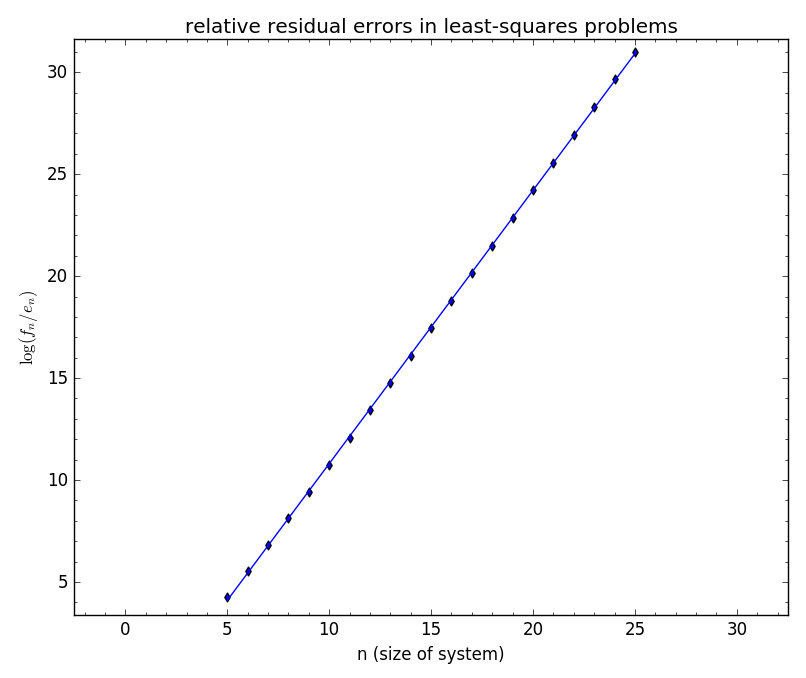
\includegraphics[width=0.8\linewidth]{2e_graph.png}
    \caption{A plot of relative errors of the least squares solutions
    found via back-substitution (with relative residual $e_n$ and
    via QR of normal equations (with relative residual $f_n$.}
\end{center}
\end{figure}
\end{small}

The slope of our fitted line is approximately 1.3412, and thus we conclude
\[
        \frac{f_n}{e_n} \propto C^n \; \text{with} \; \log(C) \approx 1.3412
        \Rightarrow C \approx 3.823
    \]
\item We have the calculation (using results given on the hw spec)
    \begin{align*}
        \norm{Ax-b}_2 &= \norm{Ax - (A + \delta A) x }_2 \\
                      &= \norm{(-\delta A) x}_2 = \norm{\delta A }_2
                          \approx \norm{(\delta A) A^{-1} b }_2 \\
                      \end{align*}
                      and so
    \begin{align*}
            e_n       := \frac{\norm{Ax-b}_2}{\norm{b}_2 }
                      \approx \frac{\norm{(\delta A) A^{-1}b}_2}{\norm{b}_2}
                      \le \frac{\norm{\delta A}_2 \norm{A^{-1}}_2 \norm{b}}{\norm{b}_2}
                      &= \norm{\delta A}_2 \norm{A^{-1}}_2 \\
                      &\approx \epsilon_M \norm{A}_2 \norm{A^{-1}}_2 \\
                      &= \epsilon_M \kappa_2(A)
    \end{align*}
    \[
            \Longrightarrow \qquad \boxed{e_n \approx \epsilon_M \kappa_2(A)}
        \]

    \item We have the calculation (all norms are 2-norms)
        \begin{align*}
            \norm{Ax-b} &= \norm{A^{-T}A^{T}\left(Ax - b\right)} \\
                        &= \norm{A^{-T}\left(A^TAx - A^Tb\right)} \\
                        &= \norm{A^{-T}\left(A^TAx - \left(A^TA + \delta A\right)x\right)} \\
                        &= \norm{A^{-T}\left(\delta A\right)x}
            \end{align*}
            and so
            \begin{align*}
                f_n = \frac{\norm{Ax-b}}{\norm{b}}
                &= \frac{\norm{A^{-T}\left(\delta A\right)x}}{\norm{b}} \\
                &\approx \frac{\norm{A^{-T}\left( \left(\delta A\right)
                    \left(A^TA\right)^{-1}A^Tb\right)}}{\norm{b}} \\
                    &\leq \frac{\norm{A^{-T}} \norm{\delta A} \norm{\left(A^TA\right)^{-1}} \norm{A^T}
                \norm{b}}{\norm{b}} \\
                &= \norm{A^{-T}}\norm{A^T} \norm{\delta A} \norm{\left(A^TA\right)^{-1}}  \\
                &= \kappa(A^T) \norm{\delta A} \norm{\left(A^TA\right)^{-1}} \\
                &\approx \kappa(A^T) \left(\epsilon_M \norm{A^TA}\right)\norm{\left(A^TA\right)^{-1}} \\
                &= \epsilon_M \cdot \kappa\left(A^T\right) \kappa\left(A^TA\right) \\
                &= \epsilon_M \left[\kappa(A)\right]^3
            \end{align*}
    \[
            \Longrightarrow \qquad \boxed{f_n \approx \epsilon_M \left[\kappa_2 (A) \right]^3}
        \]
    \item
        Using parts \textbf{(e)},\textbf{(f)}, we can estimate
        \[
    \frac{f_n}{ e_n} \approx \frac{\epsilon_M \left[\kappa_2 (A) \right]^3}{\epsilon_M \kappa_2(A)}
        = \left[\kappa_2(A)\right]^2
    \]
    Using the estimate $\kappa_2(A) \approx 2^n$ for the particular system of size $n$ we generated in part
    \textbf{(b)}, this approximation is $2^{(2n)}$.
    In the language of part \textbf{(d)}, this implies $C\approx 4$, as compared to the estimate of $3.8$ found by our program. This is absolutely satisfactory given the multiple layers of approximation used to calculate our theoretical result, as well as the fitting of our line.
\end{enumerate}
\end{prob}
\hrulefill % ___________________________________________________________
\newpage



\section{Appendix}

\lstinputlisting{../givens.py}
\clearpage
\lstinputlisting{../lsq_demo.py}
\end{document}
